\documentclass[12pt, french]{article}
\usepackage{fontspec}
\setmainfont{Arial}
\usepackage{wrapfig}
\usepackage[french]{babel}

\usepackage{setspace}
\singlespacing

% normal box
\newcommand{\sqboxs}{1.2ex}% the square size
\newcommand{\sqboxf}{0.6pt}% the border in \sqboxEmpty
\newcommand{\sqbox}[1]{\textcolor{#1}{\rule{\sqboxs}{\sqboxs}}}

%\usepackage[none]{hyphenat}
%\usepackage{hyphenat}

\usepackage{graphicx}
\usepackage{caption}
%\usepackage[T1]{fontenc}
%\usepackage[utf8]{inputenc}
\usepackage{lmodern}
\usepackage{geometry}
\geometry{
	a4paper,
	left=20mm,
	right=20mm,
	top=25mm,
	bottom=25mm,
}

\usepackage{pgfgantt}
\usepackage{eurosym}

\usepackage{pdfpages}


\usepackage{subcaption}

\usepackage[unicode=true,pdfusetitle,bookmarks=true,bookmarksnumbered=false,bookmarksopen=false,
breaklinks=false,pdfborder={0 0 0},backref=false,colorlinks=true,urlcolor=magenta]{hyperref}

\usepackage{multibib}
\newcites{article,conf,confnoproc}{{Articles dans des revues internationales à comité de lecture
	},{Communications dans des congrès internationaux à comité de lecture et actes
		publiés},{Communications dans des congrès internationaux sans comité de lecture}}


\newcommand{\review}[1]{\textcolor{blue}{#1}}

\graphicspath{{images/}}

\author{Andrea Brugnoli \\ 
	\hspace{2.8pt} Docteur ISAE-SUPAERO 2020\\
	Ingénieur ISAE-SUPAERO 2017}
\title{Plan de Recherche}

\date{}

\begin{document}
	
	\maketitle
	
	\begin{figure}[h]
		\centering
		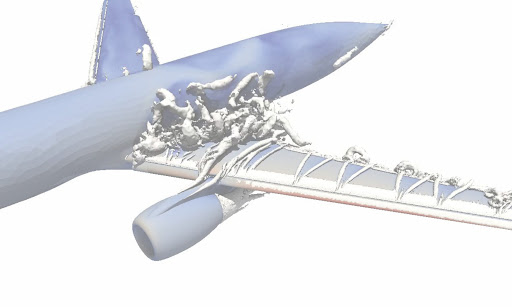
\includegraphics[width=.95\textwidth]{3Dplane.jpg}
		\captionsetup{labelformat=empty}
		\caption{Source: \href{http://www.fenics-hpc.org/}{FEniCS-HPC website}}
	\end{figure}
	
	
	
	
	
	\thispagestyle{empty}
	
	\newpage
	
	\tableofcontents
	\newpage
	
	
	\section{Les grandes lignes}
	
	Le but de mon projet de recherche consiste à mettre en place des méthodes numériques
	pour accélérer la simulation des problèmes d'interaction fluide-structure (IFS), par rapport au temps de calcul requis pour une simulation haute-fidélité. Il sera donc possible d'intégrer des modèles plus économiques, qui pourront remplacer des simulations très coûteuses. Cela permettra également de faciliter le design optimisé des composantes du système et la prise de décision. À la différence de plusieurs méthodes proposées dans la littérature, l'impératif est la fidélité à la structure physique du problème.  Cette structure est le plus souvent ignorée par les algorithmes de réduction, qui traitent les simulations comme des boîtes noires. Les modèles réduits respectueux de la physique sont beaucoup plus précis que ceux qui ne la garantissent pas et leur utilisation pourra radicalement améliorer les techniques normalement utilisées pour l'optimisation. Pour réaliser son ambition, ce projet vise à utiliser des formalismes mathématiques récents pour la modélisation multiphysique et la digitalisation des modèles. Les outils capables de prédire le comportement des systèmes complexes ont une importance fondamentale pour nous aider à affronter les prochains défis technologiques et sociétaux. Le fait que cette année le Prix Nobel de Physique ait été attribué à trois chercheurs travaillant sur ce sujet\footnote{\url{https://www.nobelprize.org/prizes/physics/2021/summary/}} confirme
	l'importance et l'actualité de cet axe de recherche.
	
	
	\section{Développement du projet scientifique}
	
	\subsection{Les problèmes multiphysiques}
	L'ingénierie computationnelle est une science récente, multidisciplinaire et en expansion rapide. Son but consiste à mettre en place des modèles mathématiques et numériques pour prédire le comportement des systèmes complexes. Cela permet de concevoir des systèmes ex novo ou bien de détecter des fautes pendant le cycle de vie des composants, sans devoir utiliser des tests expérimentaux très co\^{u}teux. Ce domaine est en expansion rapide car aujourd'hui on dispose d'ordinateurs plus puissants et surtout parce que les algorithmes ont été optimisés pour être plus rapides, robustes et faciles à utiliser. Toutefois les problèmes multiphysiques, qui sont centraux dans les applications industrielles, sont extrêmement compliqués à traiter. Cela est d\^u d'une part à la difficulté associée au traitement des différentes physiques et d'autre part à la taille des systèmes obtenus, qui nécessitent plusieurs jours, voire plusieurs semaines, pour être résolus à l'aide d'un supercalculateur \cite{keyes2013}. Ces problématiques posent des barrières pour l'utilisation des modèles numériques en industrie. 
	
	
	\subsection{Outils scientifiques du projet}
	
	
	\paragraph{\large Un formalisme unificateur pour la modélisation des systèmes dynamiques\\}
	Un formalisme mathématique très prometteur pour traiter les problèmes multiphysiques est le formalisme port-Hamiltonien \cite{vanderSchaft2002}, basé sur la mécanique Hamiltonienne et les graphes de liaisons pour la modélisation des systèmes dynamiques (cf. l'annexe \ref{sec:pHreview} pour plus de détails sur cette théorie). Au c\oe{}ur de ce formalisme, il y a l'idée que tout système physique peut être décrit d'une manière modulaire. C'est-à-dire à partir des ses composantes simples, interagissant entre eux et avec le milieu environnant à travers des portes. Les portes d'interaction contiennent l'information relative au flux d'énergie entre les différents composants et entre différents domaines physiques: mécanique, électromagnétisme ou dynamique des fluides. La conception modulaire est centrale dans l'ingénierie, car le design de tout système technologique est fait à partir des éléments simples qui sont assemblés pour donner lieu à la complexité qui nous entoure. Prenez par exemple un avion, un hélicoptère, un satellite (cf. Fig. \ref{fig:satellite}) : pour pouvoir optimiser leur design il est indispensable de disposer d'un outil de modélisation capable de décomposer la complexité de manière à retrouver les différents composants clés. Le fait d'utiliser un outil de modélisation unifié représente une nouveauté essentielle de ce projet. Cela pourra permettre la création d'une infrastructure commune pour les outils numériques à la base de la digitalisation, afin de faciliter son adoption dans l'industrie.
	
	\begin{figure}[hb]
		\centering
		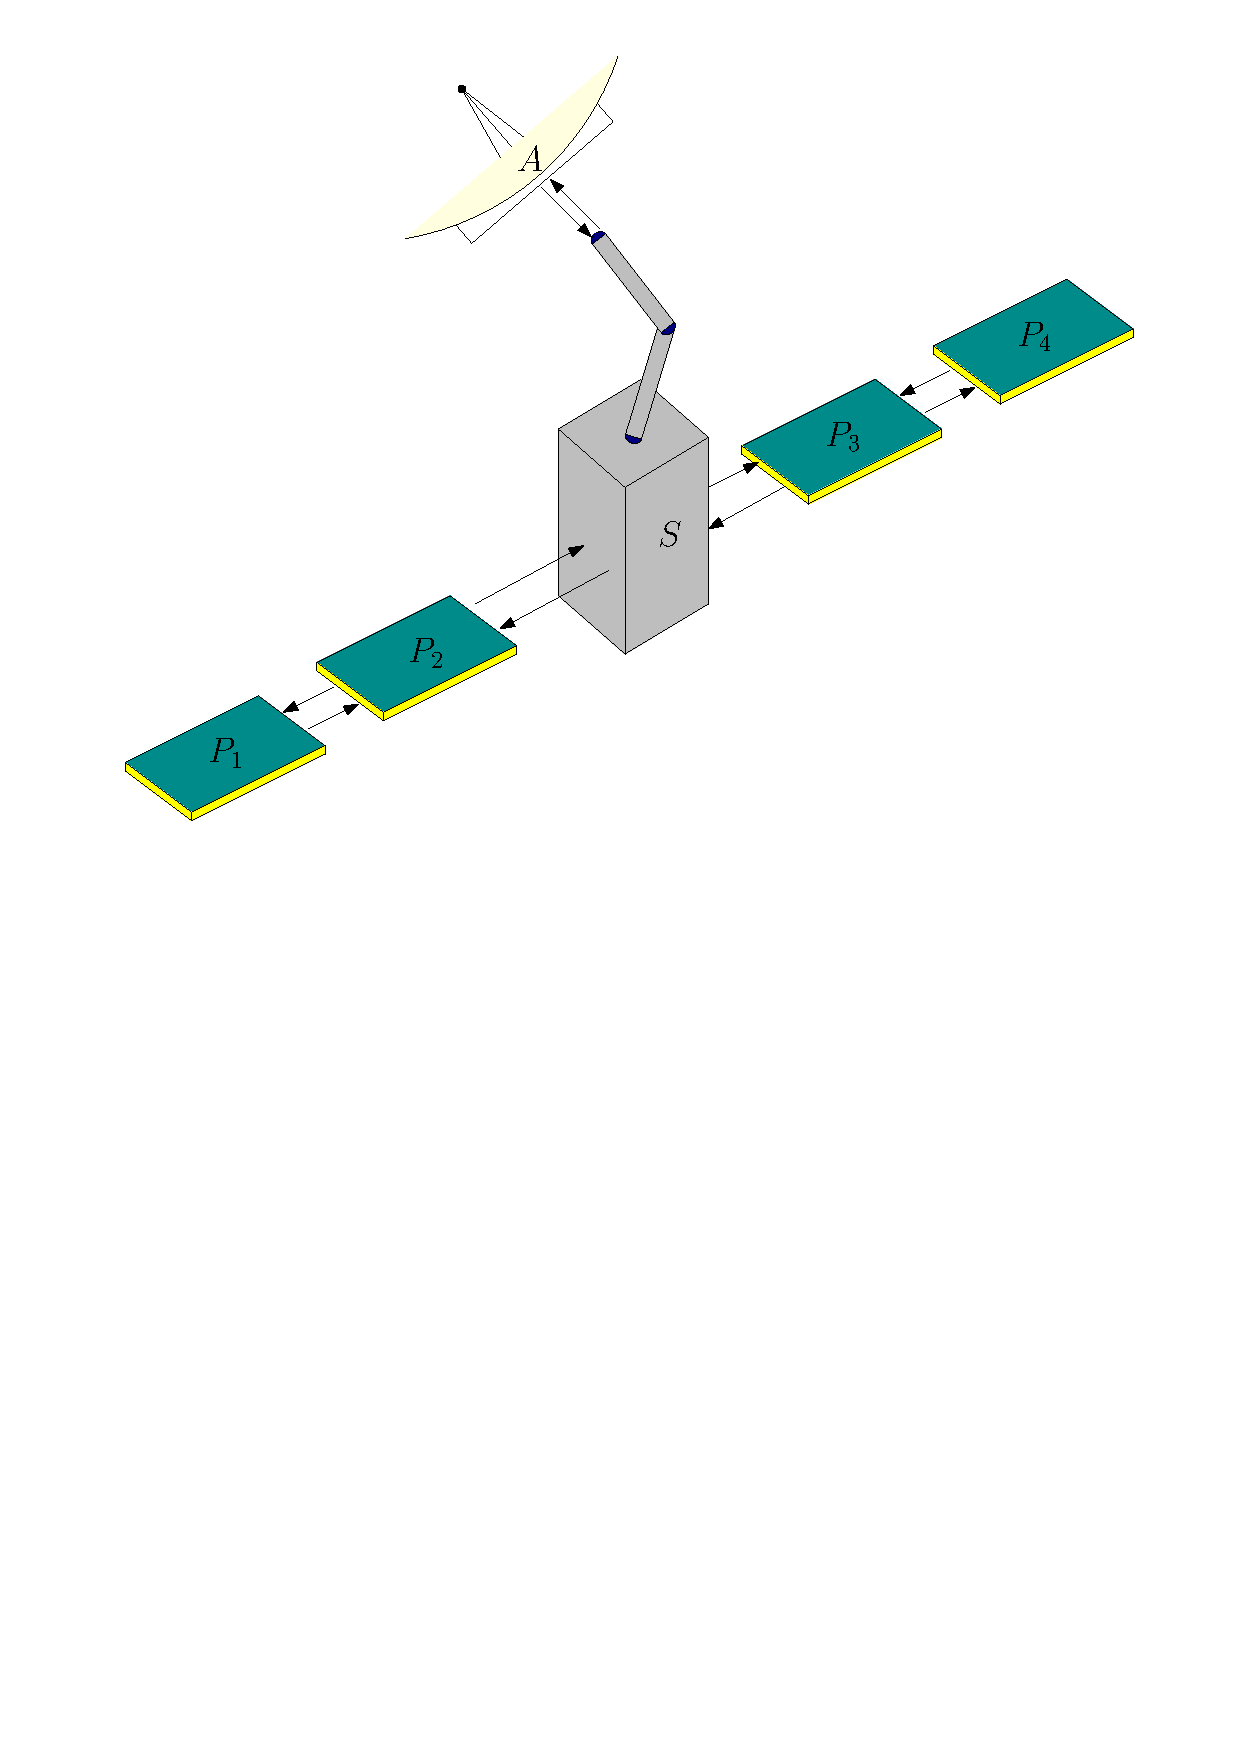
\includegraphics[width=.55\textwidth]{satellite.pdf}
		\caption{Schéma modulaire représentant un satellite de télécommunication.}
		\label{fig:satellite}
	\end{figure}
	
	\paragraph{\large Une méthodologie structurée pour la discrétisation \\}
	Les algorithmes numériques utilisés en industrie sont adaptés à la nature physique du problème. Pour la mécanique des solides, la méthode des éléments finis est privilégiée par les ingénieurs. Pour la dynamique des fluides, les volumes finis sont majoritairement utilisés car il garantissent le respect des lois de conservation. Quand il faut utiliser ces deux approches simultanément, leur couplage pose plusieurs défis. Les deux méthodes utilisent des degrés de liberté différents (i.e. différentes entités topologiques du maillage) et l'interconnexion introduit forcément des erreurs. Un outil de modélisation général nécessite une méthode de discrétisation également générale, capable de  garantir la possibilité d'interconnecter des physiques distinctes. Récemment, un formalisme unificateur pour la discrétisation des équations à dérivées partielles  à été développé  \cite{arnold2006acta}. Cette théorie mathématique, appelée la méthode des éléments finis en calcul extérieur or FEEC\footnote{Le calcul extérieur représente une généralisation du calcul vectoriel basée sur la géométrie différentielle.}, a permis des développements importants pour la discrétisation des équation aux dérivées partielles issues de la physique. Elle à été appliquée avec succès au cas de la mécanique des solides, la dynamique des fluides et l'électromagnétisme et elle représente un outil puissant pour les applications multiphysiques. La portée de cette théorie est illustrée par le fait que le Royaume-Uni a décidé d'utiliser cette nouvelle méthode pour renouveler les codes de calcul pour la météorologie\footnote{Le site \url{https://www.metoffice.gov.uk/research/news/2021/gungho-and-lfric-10th-anniversary} donne un aperçu du projet. Le lecteur intéressé peut aussi consulter les planches  \url{https://www.ecmwf.int/sites/default/files/elibrary/2016/16815-introduction-lfric-project.pdf}}.
	
	\paragraph{\large L'intelligence artificielle pour obtenir des modèles réduits\\}
	Toute méthode de discrétisation, même la plus sophistiquée, amène à des systèmes dont la taille dépasse facilement le million d'inconnues. Pour pouvoir optimiser le design des composantes mécaniques, il faut simuler ces modèles plusieurs fois. Cela amène à des coûts computationnels prohibitifs même pour les entreprises dotés des centres de calcul les plus avancés. Il est donc indispensable d'introduire des méthodes de réduction, qui sont censées construire un modèle plus simple, capable néanmoins de retenir les propriétés principales du système de départ. La grande majorité de ces méthodes suppose que l'on puisse obtenir un système réduit à travers une méthode essentiellement linéaire, i.e. la Décomposition Orthogonale en Valeurs Propres (POD) \cite{shinde2019,tello2020fluid}. Cette hypothèse n'est pas valable pour tout système exhibant un comportement non-linéaire et conduit à surestimer la dimension du système réduit. Grâce aux progrès récents dans le domaine de l'Intelligence Artificielle (IA), de nouvelles méthodes permettent d'obtenir des modèles réduits plus performants. Par exemple, des chercheurs ont proposé une architecture basée sur les réseaux neuronaux convolutifs \cite{lee2020} pour obtenir des modèles beaucoup plus rapides (d'un facteur 100 environ) par rapport aux discrétisations haute fidélité. Leur technique représente une extension non linéaire des méthodologies couramment utilisées. Les résultats obtenus démontrent le gain de performances qu'il est possible d'obtenir en utilisant les réseaux neuronaux convolutifs (cf. Fig. \ref{fig:deepROM}).
	
	\begin{figure}[t]
		\begin{subfigure}[t]{0.465\textwidth}
			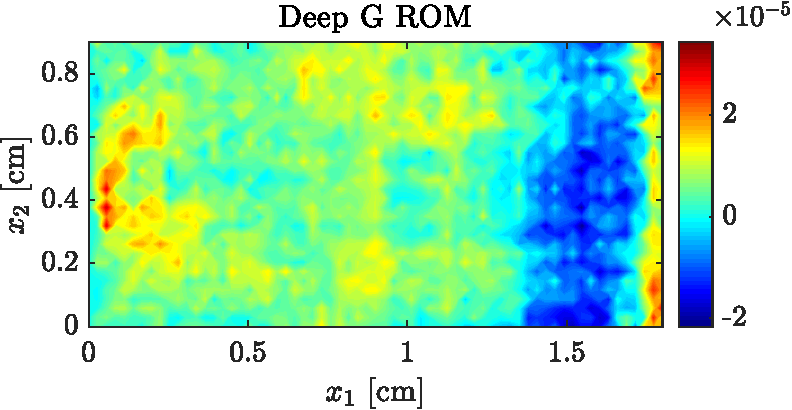
\includegraphics[width=\columnwidth]{DGROM_T_param1.pdf} 
			\caption{Modèle réduit avec réseaux des neurones.}
			\label{fig:DG_ROM}
		\end{subfigure}\hfill
		\begin{subfigure}[t]{0.48\textwidth}
			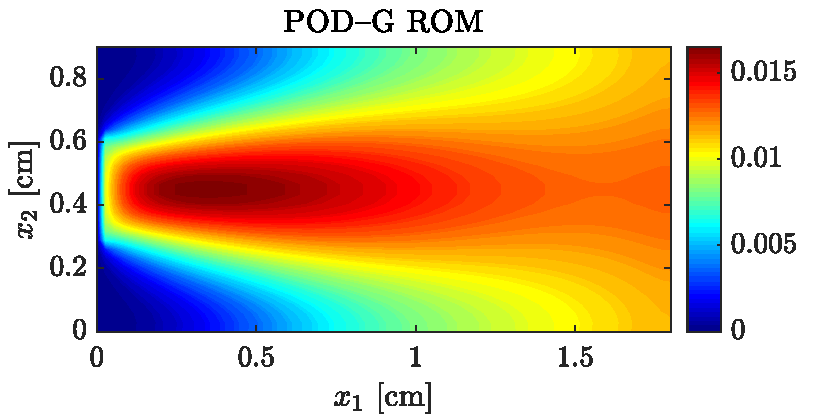
\includegraphics[width=\columnwidth]{GROM_T_param1.pdf}%
			\caption{Modèle réduit avec la méthode linéaire POD.}
			\label{fig:POD_ROM}
		\end{subfigure}
		\caption[]{Erreur des modèles réduits sur le champ de température pour un problème de convection-diffusion-réaction. En utilisant un réseau neuronal convolutifs pour générer une variété non linéaire (cf. Fig. \ref{fig:DG_ROM}) l'erreur associée à la réduction  est drastiquement réduite, de $10^{-2}$ à $10^{-5}$, par rapport à la méthode POD (cf. Fig. \ref{fig:POD_ROM}). Reproduit de \cite{lee2020} avec permission.}%
		\label{fig:deepROM}%
	\end{figure}
	
	
	\subsection{Verrous scientifiques et lots de travaux pour les adresser}
	Le premier défi est liée \`a la résolution des systèmes couplés multiphysiques.  Dans l'industrie des méthodes différentes sont habituellement utilisées pour simuler des physiques distinctes. Par conséquent, il est souvent nécessaire d'integrer différents solveurs et logiciels pour pouvoir simuler ces problèmes. Cela amène \'a une complexification des procédures industriels. Par ailleurs, le couplage numérique ne représente pas correctement les flux d’énergie. \\
	
	Le premier lot de travail (\textbf{WP1}) cherche à résoudre les problématiques liées au couplage multiphysique, d'une manière a garantir le respect des fluxes d'energie entre différentes physiques. Ces modèles numériques devront retenir les propriétés physiques du problème (conservation d’énergie globale, traçage des échanges d’énergie entre les différents sous-systèmes, invariants du problème). \\
	
	\begin{itemize}
		\item \textbf{WP1} : Développement d'algorithmes numériques haute-fidélité pour des problèmes d'interactions fluide-structures, basés sur les élément finis en calcul extérieur et le formalisme port-Hamiltonien. \\
	\end{itemize}
	
	L’utilisation d’un paradigme de modélisation unifié permettra d’effectuer les couplages de manière à respecter la physique.\\
	
	Le second verrou scientifique concerne l'intégration des techniques issues de l'IA pour obtenir des modèles réduits physiques. Il s'agit d'un thème de recherche récent mais en expansion rapide. Pour le moment, l'intelligence artificielle est utilisée majoritairement pour automatiser des taches simples, comme la classification automatique des images, du texte, des vidéos, etc. Malgré les exploits récents des algorithmes capables de surpasser les hommes dans le jeux de société comme les échecs ou le go, l'utilisation de l'IA pour la physique computationelle est encore dans un état embryonnaire. Il est extrêmement important de comprendre les avantages et limitations de ces techniques pour les intégrer à l'ensemble des outils numériques qui ont déjà fait leurs preuves dans la modélisation physique. \\
	
	Le deuxième lot de travail (\textbf{WP2}) a comme but la génération des modèles réduits capables d'incorporer la physique du problème d'une manière interprétable. \\
	
	\begin{itemize}
		\item \textbf{WP2} : Méthodes de réduction garantissant le respect de la structure physique implémentées en utilisant les réseaux des neurones.\\
	\end{itemize}
	
	Ce lot de travail consentira d'obtenir des modèles de petite dimension, prêts à être utilisés pour la partie optimisation.\\ 
	
	L'optimisation et les études paramétriques sont typiquement effectuées sur les
		modèles de substitution en industrie, car optimiser directement les modèles fins entraîne des coûts computationels absolument prohibitifs. Il est très difficile de savoir \`a l'avance quelle méthode utiliser pour générer un modèle de substitution un certain problème physique \cite{lancaster2018}. La fiabilité des ces modèles est également difficile \'a prévoir, vu que le sens physique est détruit par la procédure de réduction. \\
	
	Le dernier objectif du projet est de démontrer que les modèles réduits obtenus dans le \textbf{WP2} pourront servir de modèles de substitution plus fiables que ceux qui sont normalement utilisés. Dans le troisième lot de travail (\textbf{WP3}) les modèles réduits seront donc employés pour optimiser le design mécanique des structures et pour le contrôle optimal des structures flexibles. Cette étape permettra d’évaluer la validité et l’efficacité des modèles réduits par rapport aux simulations fines. \\
	
	\begin{itemize}
		\item \textbf{WP3} : Utilisation des modèles réduits pour l'optimisation et le contrôle optimal et comparaison avec les  modèles haute-fidélité. \\
	\end{itemize}
	
	La résolution de ces trois macro-tâches permettra de mieux comprendre le compromis entre le temps de calcul et la précision pour des applications d'intérêt industriel. Potentiellement, les techniques développées dans ce projet pourront fournir des solutions plus performantes que celles normalement utilisées en industrie. 
	
	
	\appendix
	
	\section{Les systèmes port-Hamiltoniens}\label{sec:pHreview}
	
	Dans cette annexe la théorie des systèmes port-Hamiltoniens est rapidement présentée. La discussion reprends l'introduction du livre \cite{van2014port}. \\
	
	La théorie des systèmes port-Hamiltoniens rassemble différentes traditions dans la modélisation et l'analyse des systèmes physiques. Premièrement, du point de vue de la modélisation, elle trouve son origine dans la modélisation basée sur les ports, lancée par Henry Paynter à la fin des années 50. Ce formalisme vise à fournir un cadre unifié pour la modélisation de systèmes appartenant à différents domaines physiques (mécanique, électrique, hydraulique, thermique, etc.). Ceci est réalisé en reconnaissant l'énergie comme \textit{lingua franca} entre les domaines physiques, et en identifiant des composants idéaux capturant les principales caractéristiques physiques (stockage d'énergie, dissipation d'énergie, routage d'énergie, etc.).  \\
	
	Une deuxième origine de la théorie des systèmes port-Hamiltoniens est la mécanique géométrique. Dans ce branche de la physique mathématique la formulation Hamiltonienne de la mécanique classique est formalisée de manière géométrique. Le paradigme de base
	de la mécanique géométrique consiste à représenter la dynamique Hamiltonienne d'une manière intrinsèque, c'est à dire sans introduire des coordonnées, en utilisant un espace d'état doté d'une structure symplectique ou de Poisson, ainsi que d'une fonction Hamiltonienne représentant l'énergie. Cette
	approche géométrique a conduit à une théorie élégante et puissante pour
	l'analyse du comportement dynamique des systèmes Hamiltoniens, affichant leurs caractéristiques, telles que les symétries et quantités conservées, de manière transparente. \\
	
	\begin{figure}[hbt]
		\begin{center}
			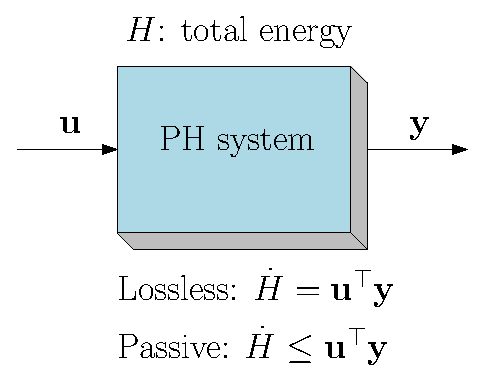
\includegraphics[width=0.35\textwidth]{sketch_PH.eps}
		\end{center}
		\caption{Un système port-Hamiltonien est un système Hamiltonien sujet \`a l'interaction avec le monde extérieur.}
		\label{fig:sketchPH}
	\end{figure}
	
	Enfin, un troisième pilier sous-jacent au cadre des systèmes port Hamiltoniens est la théorie des systèmes et du contrôle, o\'u les systèmes dynamiques sont décrits comme étant ouverts à l'interaction avec l'environnement (par exemple via des entrées et des sorties, cf. Fig. \ref{fig:sketchPH}) et comme étant susceptibles d'être contrôlées activement. \\
	
	
	Une différence principale entre la théorie des systèmes port-Hamiltoniens et la mécanique géométrique réside dans le fait que pour la première la structure géométrique sous-jacente n'est pas nécessairement la structure symplectique de l'espace des phases, mais est en fait déterminée par la structure d'interconnexion du système.  En ce sens la théorie port-Hamiltonien fusionne intrinsèquement la géométrie avec la théorie des réseaux, grace \`a la notion de structure de Dirac. Une propriété clé des structures de Dirac est le fait que leur composition est à nouveau une structure de Dirac. Cela a pour conséquence cruciale que l'interconnexion des systèmes port-Hamiltoniens par leur ports est à nouveau un système port-Hamiltonien (cf. Fig. \ref{fig:intPH}). Une autre extension de la théorie des systèmes port-Hamiltoniens par rapport à la mécanique géométrique est l'inclusion d'éléments dissipateurs d'énergie, qui sont largement absents dans les systèmes Hamiltoniens classiques. Cette inclusion élargit considérablement le domaine d'application des systèmes port-Hamiltoniens par rapport à celui des systèmes Hamiltoniens classiques. \\
	
	La modélisation port-Hamiltonien apparaît comme une théorie générale pour la modélisation des systèmes physiques complexes rencontrés dans de nombreux domaines de l'ingénierie.
	
	
	\begin{figure}[tbh]
		\begin{subfigure}[t]{0.45\textwidth}
			\includegraphics[width=\columnwidth]{sketch_PH_gyrator.eps} 
			\caption{Gyrateur}
			\label{fig:pHsys_gyr}
		\end{subfigure}\hfill
		\begin{subfigure}[t]{0.45\textwidth}
			\includegraphics[width=\columnwidth]{sketch_PH_transformer.eps}%
			\caption{Transformer}
			\label{fig:pHsys_tran}
		\end{subfigure}
		\caption[]{Interconnexion des deux systèmes port-Hamiltonien: ces deux type d'interconnexion sont telles \`a préserver les échanges de puissance entre les deux systèmes.}%
		\label{fig:intPH}%
	\end{figure}

	\section{Le code SCRIMP}\label{sec:SCRIMP}
	Le code SCRIMP (Simulation and ContRol of Interactions in Multi-Physics) est un projet Python pour l'approximation numérique d'équations aux dérivées partielles contrôlées \`a la frontière en utilisant le formalisme port-Hamiltonien. La principale motivation derrière le développement de SCRIMP était de fournir un cadre facile à utiliser pour la solution numérique des systèmes port-Hamiltoniens de dimension infinie à des fins à la fois de recherche et d'enseignement. Les approximations numériques avec des discrétisations sont gérées par le logiciel d'éléments finis FEniCS (\url{https://fenicsproject.org/}). Des applications basés sur des équations aux dérivées partielles paraboliques ou hyperboliques sont abordées. Plusieurs cahiers sont fournis pour démontrer l'utilisation de SCRIMP dans ce cadre \url{https://zenodo.org/record/4945329\#.YflFPVvMJH5}.


	\bibliographystyle{unsrt}
	\bibliography{biblio_recherche}
	
	
\end{document}
